% Chapter 3

\chapter{Propuesta de aplicación} % Main chapter title
% \chapter{Propuesta de aplicación de modelos \glsentrytext{nlp} para el desarrollo de labores de inteligencia en escenarios de ciberterrorismo} % Main chapter title

\label{chap:proposal} % For referencing the chapter elsewhere, use \ref{Chapter1} 

%----------------------------------------------------------------------------------------

\newcommand{\nmodels}{{3 }}

La propuesta consta de a aplicación de modelos de \glsentrytext{nlp} para el desarrollo de labores de inteligencia en escenarios de ciberterrorismo por medio de \nmodels modelos, pensados para el análisis de texto en redes sociales como Twitter en aras de realizar un perfilado de ciber-criminales potenciales. Esta propuesta estará fundamentada en varias tecnologías identificadas en el \mbox{Estado-del-Arte}.

Para esto se sigue el ciclo \gls{crisp-dm}, el cual contiene 6 fases, y 4 de las cuales fueron abordadas en este proyecto: \todo{explicar por que no se siguieron las otras 2 fases}
\begin{enumerate}
\item Entendimiento del negocio (\textsl{Business understanding})
\item Adquisición de datos (\textsl{Data acquisition})
\item Modelamiento (\textsl{Modelling})
\item Despliegue (\textsl{Deployment})
\end{enumerate}

\section{Entendimiento del negocio (Business understanding)}
En el proceso de perfilado una tarea muy importante se basa en la búsqueda de pistas (como diversos ejemplos dados en \cite{mena2003investigative}), por lo que la mayor parte de este proceso confiere de tratar de encontrar patrones que confieran algún tipo de relación entre lo que es un actor y una acción, si bien no necesariamente de forma directa. Es por esto que técnicas como las que se encuentran en la minería de texto (véase la \cref{subsec:NLP}) confieren una posibilidad de realizar muchas de estas labores, tales como el \gls{clustering} (véase la \cref{subsec:clustering}) de elementos, como el caso de la \cref{fig:som-example} en la \cref{subsec:SOM}.

La necesidad cae en las agencias de seguridad que requieren de estar constantemente buscando posibles relaciones entre ataques pasados o futuros, y por tanto nuevas herramientas que permitan obtener nuevas habilidades en la esta labor son esenciales.

Finalmente, metodologías de análisis de textos a partir de fuentes abiertas, tales como en \cite{osint}, permitirían no solo obtener la información, sino que tener una forma de analizarla e incluso de predecir relaciones a partir del contenido que no es explícito.

% ================================================================
% ================================================================

\section{Adquisición de datos (Data acquisition)} \label{sec:data-acquisition}
Para esta labor de adquisición de datos, la intención es de recolectar datos de diversas fuentes, sin embargo para el alcance del proyecto se proponen dos metodologías de obtención de información de fuentes abiertas que serán explicadas en las subsecciones \ref{subsec:twitterapi} y \ref{subsec:twitterarchive}.

\subsection{Obtención de datos con API de Twitter} \label{subsec:twitterapi}
Twitter permite el acceso de datos de su plataforma por medio de códigos de autorización provistos en ella, que luego son usados para obtener la información con criterios definidos por el usuario.\todo{indicar cuales fueron los criterios de selección de tweets}

\subsubsection{Petición de autorización en Twitter}
Para realizar una petición de datos de acceso a la plataforma es necesario crear una ``App'' por medio de visitar la pagina de Administración de aplicaciones \todo{de donde? de la cuenta de un usuario regular de twitter} (o \emph{Application~Management} en ingles). Se necesita una cuenta de Twitter previamente creada.

Luego se procede a crear la App, para esto sera necesario proveer información respecto a que se hará con la aplicación y que datos requerirá esta. En este proceso es importante tener en cuenta que debido al uso masivo de información dentro de Twitter, este ha puesto restricciones al acceso por temas de privacidad e influencia, es por esto que el proceso para pedir autorización de crear una nueva aplicación debe incluir la mayor cantidad de información que provea la intención del uso. Luego de llevar a cabo la solicitud luego de aproximadamente un día le sera notificado si fue autorizado para utilizar la plataforma.

En este punto podrá crear la aplicación y generar los tokens de autorización, de los cuales requerirá de:
\begin{itemize}
\item \texttt{CONSUMER\_KEY}
\item \texttt{CONSUMER\_SECRET}
\item \texttt{ACCESS\_TOKEN}
\item \texttt{ACCESS\_SECRET}
\end{itemize}

Esta petición de datos se realiza por medio de una consulta \texttt{GET} donde la URI provee los datos como los codigos de autorización.

Dentro del directorio de Software (véase el Apéndice \ref{appendix:projectinfo}) se incluye un programa que permite la obtención de tweets con todos los meta-datos ofrecidos por la plataforma, de manera que obtiene tweets con temas relacionados especificados en un archivo de texto externo.\todo{Indicar por favor las restricciones que impone twitter en cuanto a numero de twits descargados o ventana de descarga, en esta forma de descaga gratuita. Indicar tambien las opciones pagas ofrecidas por twitter para acceder a tweets.}

\subsection{Obtención de datos con datasets públicos en Archive} \label{subsec:twitterarchive}
Otra posibilidad de obtener datos en una plataforma abierta es la de la pagina web de \textsc{Archive}\footnote{\href{https://archive.org/search.php?query=collection\%3Atwitterstream\&sort=-publicdate\&page=2}{https://archive.org/search.php?query=collection\%3Atwitterstream\&sort=-publicdate\&page=2}}.

En esta plataforma se puede descargar meses de contenido obtenido de cualquier origen en Twitter en el tiempo de un mes, aunque este información no fue obtenida con niveles altos de precisión, es decir, no se obtuvieron todos los tweets que ocurrieron durante ese mes ni tampoco fueron obtenidos en un ambiente de alta disponibilidad, por lo que no todos los tweets en ese instante fueron recolectados.

Una forma recomendada de descargar los datos de \textsc{Archive} es por medio de \emph{torrents}, que permite una descarga fiable del contenido comprimido de ese mes\footnote{Cada mes pesa aproximadamente 50GB} ya que además provee comprobación de integridad y reintento de descarga de secciones de archivos que se encuentran corruptas. Un motor de torrents Open Source es el de qBittorrent\footnote{\href{https://www.qbittorrent.org/}{https://www.qbittorrent.org/}}, y tiene implementaciones en Windows, MacOS y Linux.

Luego de haber descargado todo el archivo comprimido de tweets se puede proceder a descomprimirlo, de donde se encontrarán archivos comprimidos mas pequeños divididos por día del mes, sin embargo téngase en cuenta que descomprimir estos archivos puede llegar a pesar 500GB, por lo que una alternativa mas conveniente es de realizar un filtrado de los datos relevantes que se necesiten de manera individual\todo{este filtrado se haría antes de descargar los archivos de ARCHIVE? especificar como se puede hacer} por cada uno de esos archivos, de esta forma solo se tendría la información requerida, en vez de ruido. Para esto existe una aplicación incluida en la carpeta de Software de este proyecto con un posible uso (véase el Apéndice \ref{appendix:projectinfo}), donde también se hace uso de \cite{Tange2011a} para el procesamiento mas eficiente.

% ================================================================
% ================================================================

\section{Modelamiento (Modelling)}
Como parte de la propuesta se proponen \nmodels modelos para tratar diferentes necesidades los cuales estan representados en la \cref{fig:proposal-arch}.

\begin{figure}[H]
  \centering
  % \missingfigure{Hacer la arquitectura en yEd}
  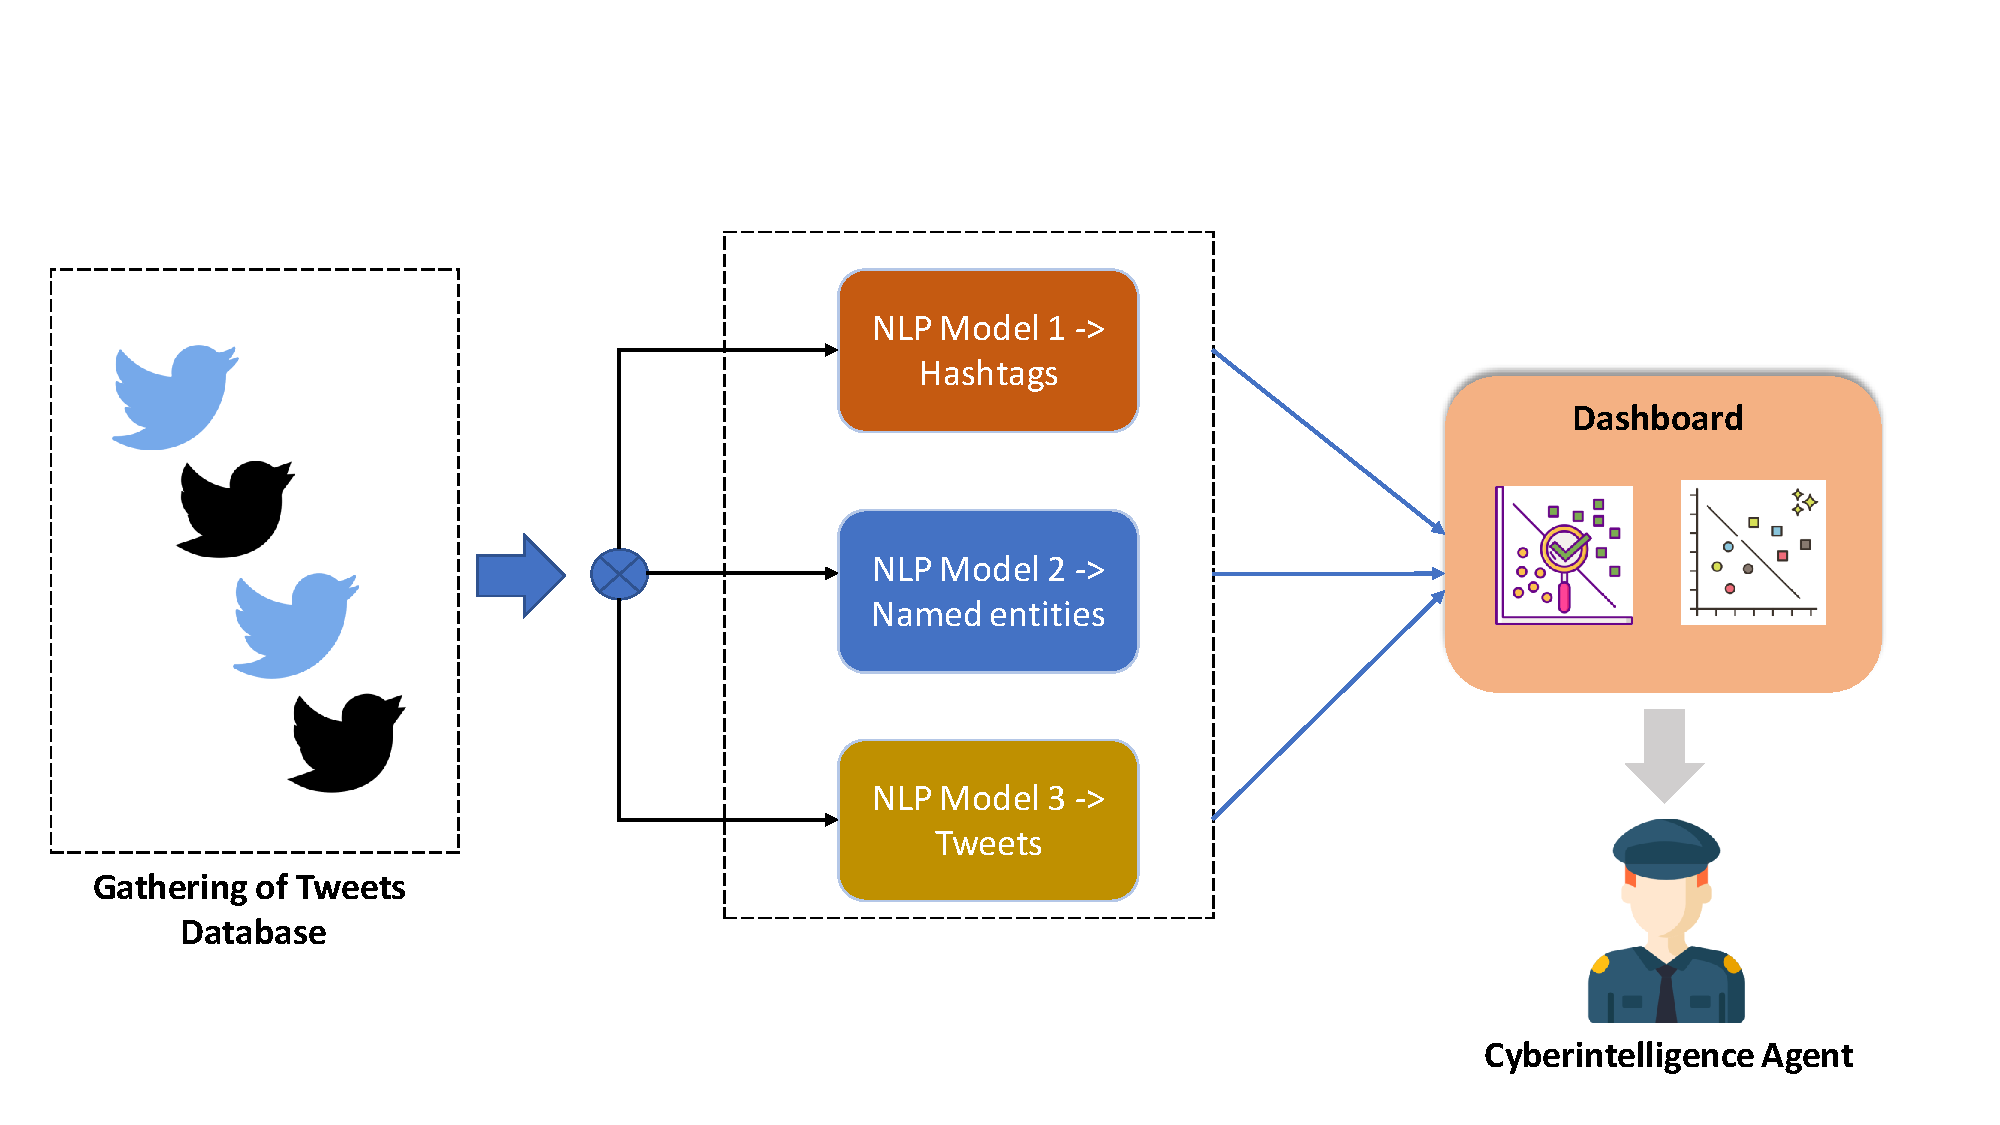
\includegraphics[width=\textwidth]{Figures/general-architecture.pdf}
\decoRule
\caption[Arquitectura de propuesta]{Arquitectura de propuesta.}
\label{fig:proposal-arch}
\end{figure}

% ================================================================
% ================================================================
% ================================================================

\subsection{Modelo 1: Predicción de etiquetas de Twitter con modelos lineales} \label{sec:twitter-prediction}
En Twitter, las publicaciones que se realizan tienen la posibilidad de incluir menciones de temas de tendencia por el conocido \emph{hashtag}, escrito como \texttt{\#Tema}, y tiene la gran utilidad de realizar una mención explicita del tema que se quiere tratar y además facilita la tarea de encontrar textos directamente relacionados con un tema.

% \todo[inline]{Antes de empezar este parrafo por favor colocar un parrafo pequeño que indique de manera explicita la pregunta de data science que se esta ressolviendo, por ejemplo ¿Cual(es) es(son) el (los) hashtag(s) de un tweet?}

Lo que se intenta solucionar con este modelo es de predecir que \emph{hashtags} deberían estar presentes en un tweet basado en la combinación de palabras que se encuentran dentro. Para esto se propone un modelo lineal que usa regresión logística y realizar una multi-clasificación con las clases siendo los \emph{hashtags} basándose del texto. Esto esta pensado con el propósito de ayudar al agente de inteligencia a identificar a que posibles tendencias pertenece un tweets de manera que pueda reconocer si es de un tema relevante para la seguridad.

Así mismo, en la literatura de \gls{nlp} es muy común el uso de diferentes representaciones de palabras o conjuntos de palabras. Una representación de palabras típicas son los \gls{bow}, donde se establece un diccionario de palabras de tamaño $N$, y donde cada palabra tiene un vector que la representa. A cada palabra se le asigna un identificador único (vector) en ese diccionario, por lo que existiría una traducción de palabra a vector y cada palabra puede ser recuperada por medio del índice, como se muestra en la \cref{eq:bow-repr1} y la \cref{eq:bow-repr2}.
\begin{equation} \label{eq:bow-repr1}
  \text{word2idx} = \Big\{(\text{word}_i, i) : \forall i \in \{1, \ldots, N\} \Big\}
\end{equation}

\begin{equation} \label{eq:bow-repr2}
  \text{idx2word} = \Big[\text{word}_i\Big], \forall i \in \{1, \ldots, N\}
\end{equation}

El lugar de donde son tomadas la palabras para representar al \gls{bow} están contenidas en un conjunto de palabras conocido como el \gls{corpus} de palabras, de esa misma manera también es posible tener \gls{corpus} de otros elementos como sentencias de texto (mas de una palabra compuesta), letras individuales, entre otras.

\todo[inline]{Actualizar seccion}

\subsubsection{Creación del \glsentrylong{corpus} de palabras}
Debido a que los textos que se encuentran en Twitter no tienen forma estructurada es necesario realizar un preprocesamiento de cada post recolectado para luego contar la frecuencia de cada palabra dentro del \gls{corpus} y así establecer las primeras $N$ palabras mas usadas que van a componer el \gls{corpus} de palabras.

Para realizar el preprocesamiento de cada texto se hacen los siguientes pasos:
\begin{enumerate}
\item Convertir todas las palabras a minúscula (e.g. \mbox{``LaTeX'' $\rightarrow$ ``latex''})
\item Reemplazar todos los caracteres especiales de texto a espacios en blanco (e.g. \mbox{``\texttt{@;,:\textbackslash n\textbackslash t\textbackslash r}'' $\rightarrow$ ``\textvisiblespace \textvisiblespace \textvisiblespace \textvisiblespace \textvisiblespace \textvisiblespace \textvisiblespace''})
\item Remover todos los símbolos extraños, es decir todo lo que no sean numeros, ni letras ni los simbolos que se encuentran normalmente en tweets (e.g. \mbox{``\texttt{\%()\*\&\$!\^}'' $\rightarrow$ ``''})
\item Remover todas las \emph{stopwords}, que son palabras que no añaden ningún valor semántico al texto \\ (e.g. \mbox{``las palabras son una forma de expresarnos'' $\rightarrow$ ``palabras forma expresarnos''})
\end{enumerate}

Luego se realiza un conteo de todas la palabras presentes dentro del \gls{corpus} de donde se sacan las $N$ primeras palabras para incluirlas en el \gls{bow}. $N$ es definido heurísticamente por el usuario.

Luego de esto se generan las etiquetas (o \emph{tags} en ingles), equivalente a este contexto como los hashtags que se toman directamente de los textos de entrenamiento, de estos también se les realiza un conteo, que servirán para la predicción de las etiquetas según el contenido del texto.\todo{Se realiza un conteo al texto de entrenamiento?}

\subsubsection{Conversión de textos a vectores}
Para realizar la conversión de textos a vectores y así poder representar un texto como un vector se procede a primera realizar una generación de identificadores para cada palabra de manera como se describió en el inicio de la \cref{sec:twitter-prediction}.

La manera en que se representa un texto en forma de vector $\vs$ es por medio de la sumatoria de los vectores que representan cada palabra como se representa en la \cref{eq:bow-word-vector-sum}, recuérdese que $\ve^{(i)}$ es un vector con un $1$ en la posición $i$ y ceros en el resto de posiciones.

\begin{equation} \label{eq:bow-word-vector-sum}
  \vs = \mathlarger{\mathlarger{\sum}}_{(\text{word}, i) \in \text{word2idx}} \ve^{(i)}, \text{word} \in d
\end{equation}

\subsubsection{Generación del conjunto de entrenamiento, validación y pruebas}
Para la generación de los conjuntos\todo{cada conjunto debería tener un tamaño diferente, cierto? por favor explicar como se generan esos conjuntos} se toman las sumatorias generadas de cada tweet en su forma de vector y se coloca en una matriz de $\mT^{m \times N}$, donde $m$ son el numero de muestras de Twitter y $N$ el tamaño del \gls{corpus}.\todo{porque m y N?}

\subsubsection{Clasificador de regresión logística}
La regresion logistica hace parte de uno de los algoritmos mas importantes en \gls{ai}, esta consiste en procesar la entrada de un modelo, que para el caso actual es lineal, que se procesa con una serie de hiper-parámetros que se denominara $\vtheta$ y la entrada del modelo como $\vx$. Se tiene que al realizar una regresión con este modelo se calcula $\vtheta^{\top} \vx$, que da como resultado un valor en $\R$ con rango indefinido. La regresión logística simbolizada como $\sigma(x)$, conocida como la función \emph{sigmoide} que es una función que para una entrada $x$ de dominio $(-\infty, \infty)$ se tiene un rango de $(0, 1)$. La \cref{eq:logits-formula} define la función \emph{sigmoide}.

\begin{equation} \label{eq:logits-formula}
  \sigma(x) = \frac{1} {1 + \exp(-x)}
\end{equation}

Equivalentemente, la regresión logística con modelos lineales se calculan como $\sigmoid(\vtheta^{\top} \vx)$ y permite realizar un suavizado de la regresión de forma que mitiga parte de los problemas de \gls{overfitting} y \gls{underfitting}, como se muestra en la \cref{fig:logits-example}.

\begin{figure}[H]
  \centering
  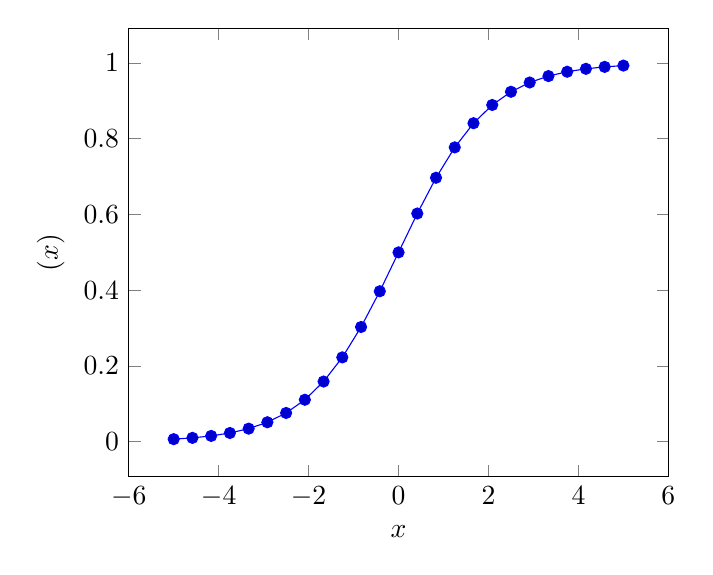
\begin{tikzpicture}
    \begin{axis}[ 
      xlabel=$x$,
      ylabel={$\sigmoid(x)$}
      ] 
      \addplot {1 / (1+exp(-x))}; 
    \end{axis}
  \end{tikzpicture}
\decoRule
\caption[Gráfica de función sigmoide]{Gráfica de función sigmoide.}
\label{fig:logits-example}
\end{figure}


\subsubsection{Multiclasificador de One vs Rest}
La multiclasificacion como es brevemente introducido en la \cref{sec:ML}, permite realizar una clasificación en $C$ clases con una entrada $\vx$. El multiclasificador de \emph{One vs Rest} realiza la clasificación por medio de distinguir la separación de una muestra $\vx_i$ en una clase $c \in \{1, \ldots, C\}$ respecto al resto de muestras, de forma que se calcula la pertenencia de la muestra $i$-\'esima en esa clase con un estimador $\vtheta_c$. De los resultados dados por cada estimador\todo{habria uno por cada clase?  por favor agregar esto para mejorar la descripción si es el caso} se estima cual es el $k$-\'esimo estimador que da el máximo valor, de donde se estima finalmente que la clase $k$ es donde pertenece la muestra.

El uso de la regresión logística se puede llevar a cabo para normalizar los resultados de los estimadores $\vtheta$, de donde el proceso para calcular el estimador consta de realizar un proceso de gradiente descendiente, que utiliza como función de costo $J: \R^n \rightarrow \R$ la \cref{eq:ovr-reg-l2costfunc} para uso de regularización con $\normltwo$ y la \cref{eq:ovr-reg-l1costfunc} para el uso de $\normlone$, según lo descrito en el manual de \cite{sklearn_api}. En ambas ecuaciones el resultado de optimizar la función de costo da como resultado el estimado final $\hat{\vtheta}$ el cual es el estimado del modelo. La función $\softplus$ es la función \emph{softplus} (véase la Notación).

\begin{equation} \label{eq:ovr-reg-l2costfunc}
  \hat{\vtheta} = \argmin_{\vtheta} J(\vtheta) = \argmin_{\vtheta} \frac{1}{2}\norm{\vtheta}_2 + C \sum_{i=1}^n \softplus(- y_i (\mX_i^{\top} \vtheta))
\end{equation}

\begin{equation} \label{eq:ovr-reg-l1costfunc}
  \hat{\vtheta} = \argmin_{\vtheta} J(\vtheta) = \argmin_{\vtheta} \norm{\vtheta}_1 + C \sum_{i=1}^n \softplus(- y_i (\mX_i^{\top} \vtheta))
\end{equation}

En el caso para realizar una multi-clasificación, la regresión logística solo puede realizar una clasificación binaria, esto es que para una entrada $\vx$, esta solo puede realizar una clasificación con salidas $y \in [0, 1]$. Debido a esta restricción, existen una metodología de multiclasificacion llamada \emph{One vs Rest}, que permite utilizar la regresión logística y realiza la multiclasificacion por medio de crear $n$ estimadores que permiten estimar cada una de las $C$ clases respecto al resto de la entrada, por cada una de los estimadores se estima cual es la clase con mayor valor en la regresión logística individual de ese estimador, la \cref{fig:ovr-algo} representa una versión simplificada del proceso.\todo{esto creo que esta repetido con el parrafo anterior. Queda redundante volver a explicar en que consiste one vs rest. Por favor incorporar al parrafo anterior para mejorar la explicacion de lo que es one vs rest y dejar la imagen que esta muy diciente}

\begin{figure}[H]
  \centering
  % \missingfigure{Hacer la arquitectura en yEd}
  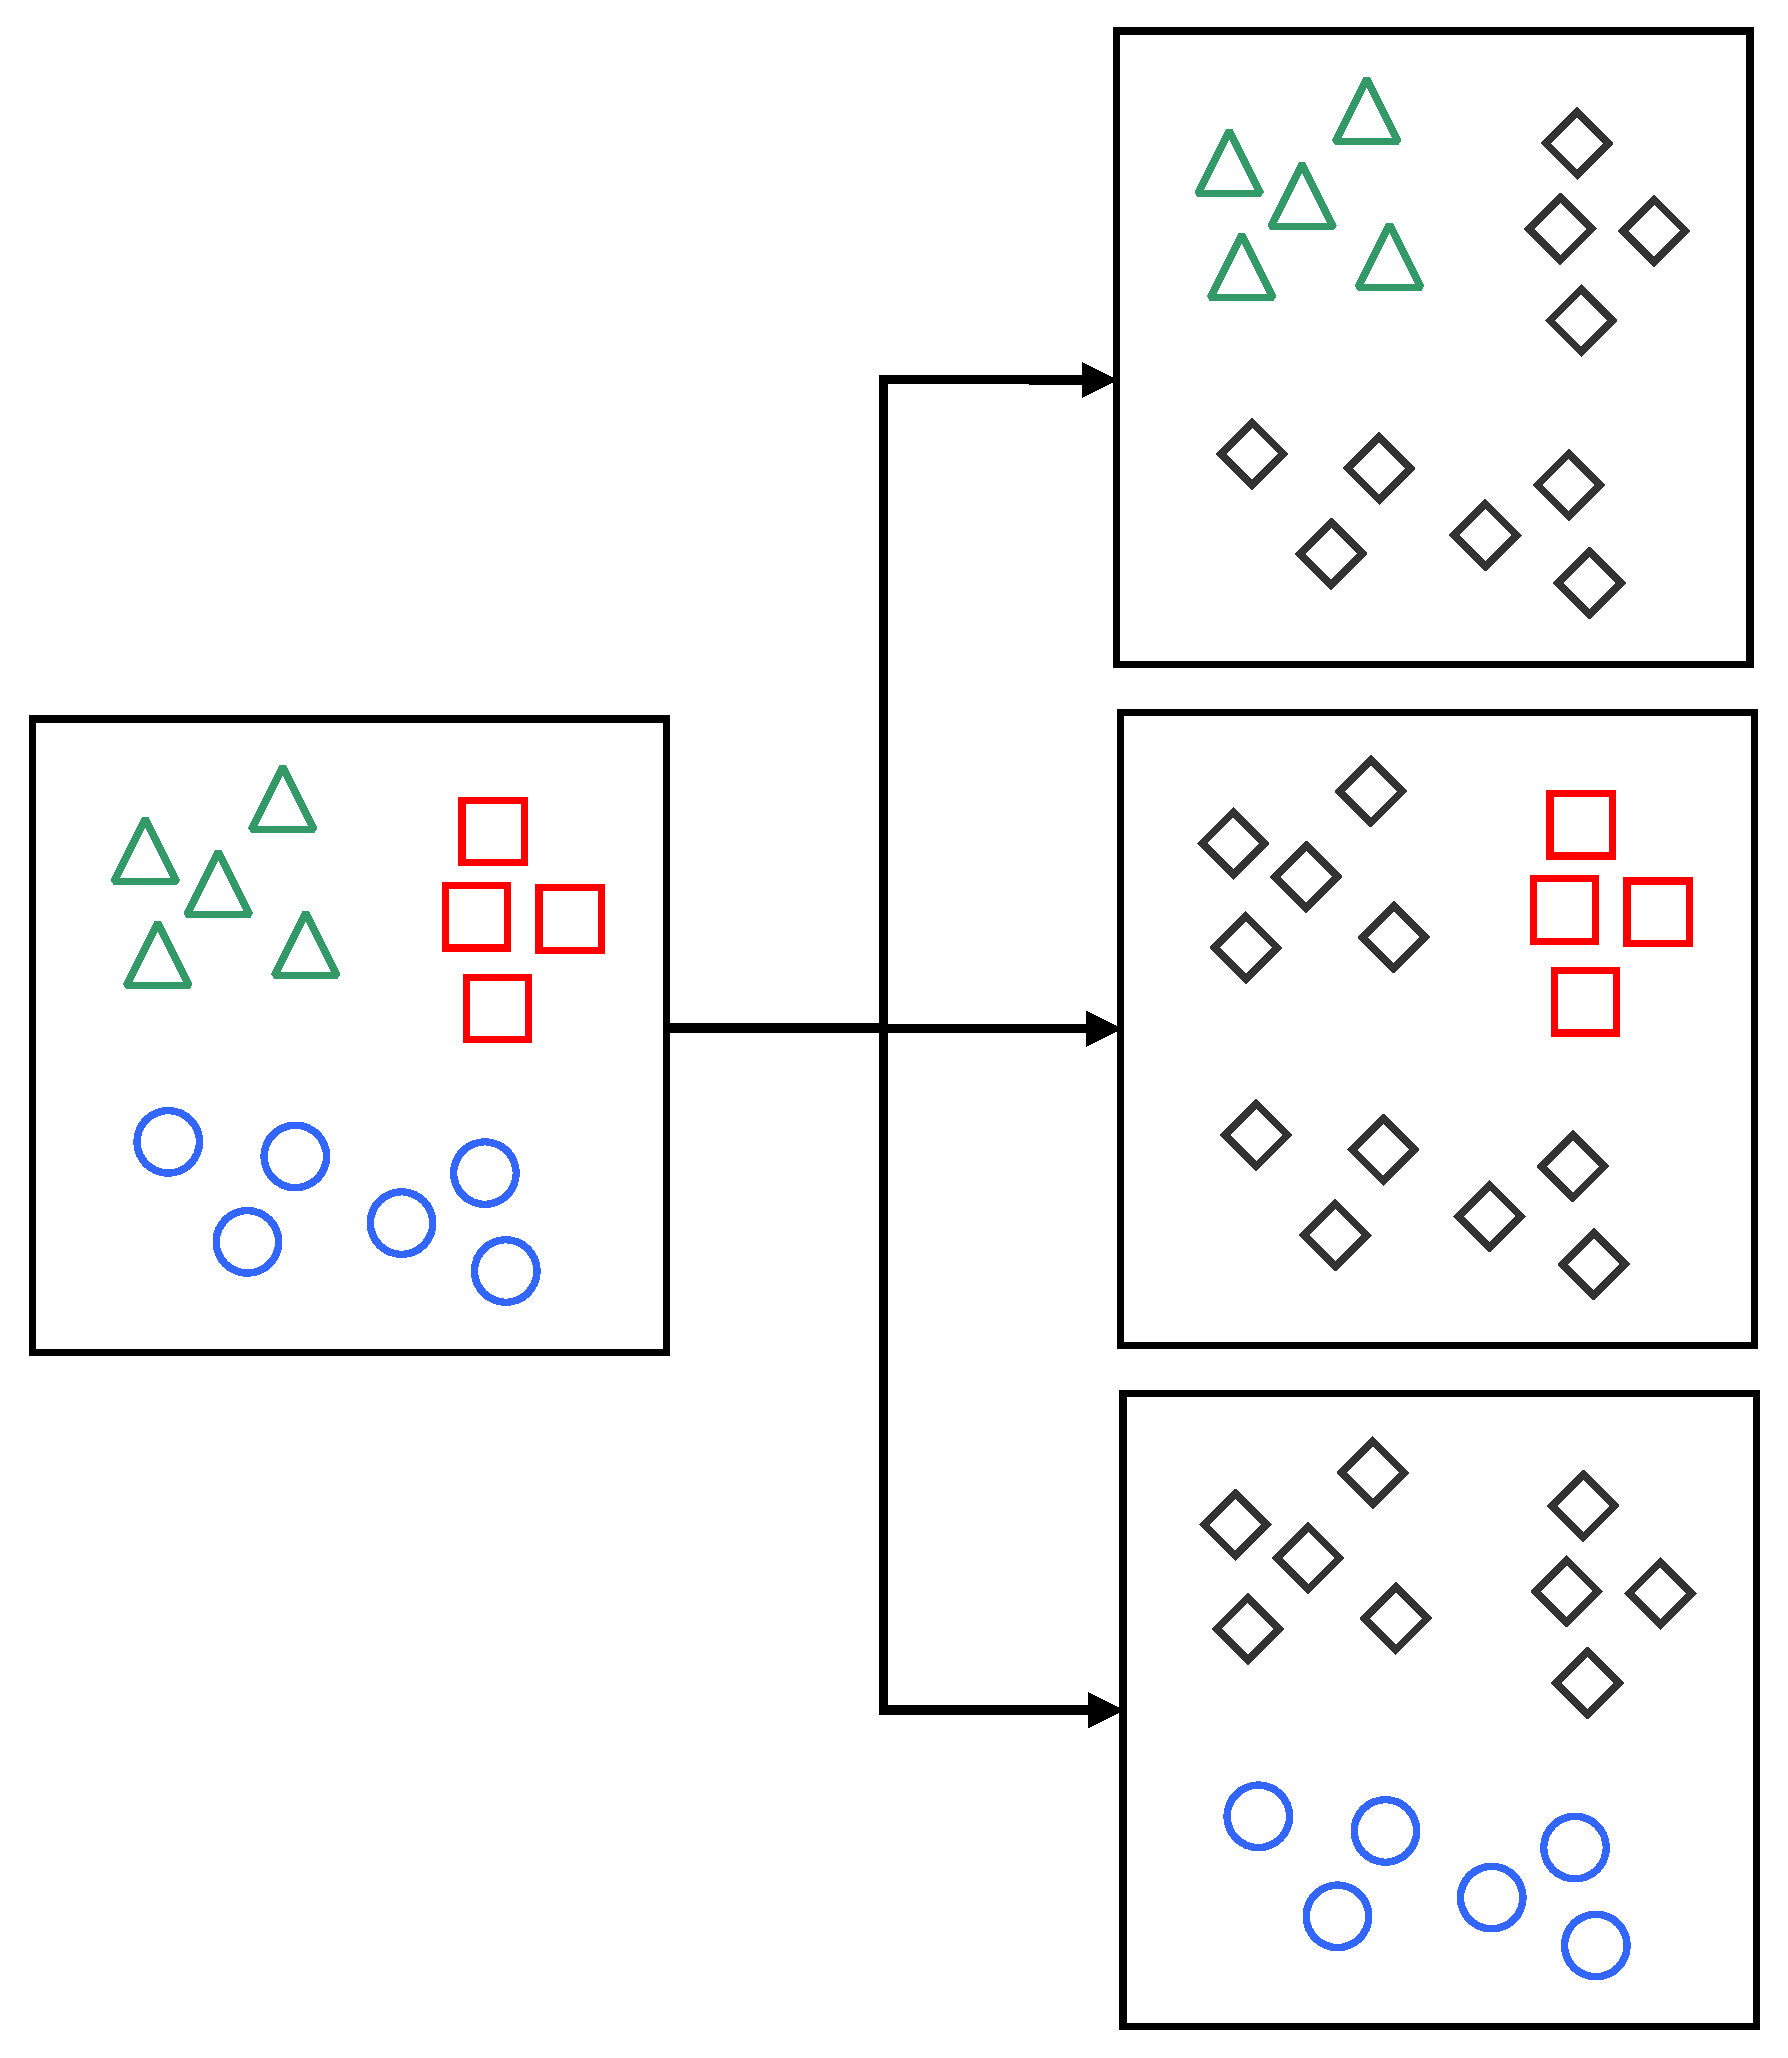
\includegraphics[width=0.5\textwidth]{Figures/one-vs-rest.pdf}
\decoRule
\caption[Algoritmo de One vs Rest]{Algoritmo de One vs Rest.}
\label{fig:ovr-algo}
\end{figure}

La manera en que se entrena cada estimador $i \in \{1, \ldots, C\}$ es por medio de optimizar el valor de la función de predicción $\hat{y}(\vx, \vtheta_i)$, $\vx \in \sX$ (\cref{eq:linear-regression-training}). Como se muestra en la \cref{eq:linear-regression-estimation}, $y$ es el valor verdadero de la estimación y $\theta_0$ se le conoce como el parámetro de ajuste del modelo.

\begin{equation} \label{eq:linear-regression-training}
  \hat{y}(\vx, \vtheta) = \vtheta^{\top} \vx = \theta_0 + \theta_1 x_1 + \cdots + \theta_n x_n
\end{equation}

\begin{equation} \label{eq:linear-regression-estimation}
  \vtheta_i = \argmin_{\vtheta_i} | \hat{y}(\vx, \vtheta_i) - y|
\end{equation}

Luego de haberse entrenado cada estimador con sus valores óptimos, se puede realizar la predicción de las clases a las que pertenece una entrada $\vx$ con la \cref{eq:ovr-prediction}.

\begin{equation} \label{eq:ovr-prediction}
  c = \argmax_i \, \sigmoid(\hat{y}(\vx, \vtheta_i))
\end{equation}

\subsubsection{Predicción de hashtags}
El uso que se le puede dar a todo lo mencionado anteriormente en esta sección es de predecir etiquetas de Twitter típicas de terrorismo a partir del texto que se encuentra en el tweet con ayuda de alguna de las representaciones de \gls{bow} o \gls{tfidf}\todo{Cual de estos dos fue utilizado finalmente en la implementación? por favor explicar}, tal como se muestra en el ejemplo de la \cref{fig:tweet-prediction}.

\begin{figure}[H]
  \centering
  \begin{tabular}{p{0.46\textwidth} p{0.05\textwidth} p{0.46\textwidth}}
    ``Really excited to add @plaidavenger to my deathlist along with Italy and @Plaid\_Obama after receiving that information.'' & $\mathlarger{\mathlarger{\mathlarger{\Rightarrow}}}$ & \textbf{\#deathlist, \#KillEveryone, \#ISIS}
  \end{tabular}
  \decoRule
  \caption{Predicción de hashtags con modelos lineales.}
  \label{fig:tweet-prediction}
\end{figure}
\todo[inline]{cada uno de estos hashtags tendría un valor diferente proveniente del respectivo estimador? cuantas clases (estimadores) se usaron en la implementación? por favor explicar e incorporar en el texto}

De manera que se determinan los $C$ hashtags de los datos de entrenamiento $\sX$ para luego poder realizar la prediccion de los hashtags a partir un texto de entrada $d$ que luego se convierte a representacion \gls{bow} o \gls{tfidf} para pasarlo por los $C$ estimadores del \emph{One vs Rest} y estimar las etiquetas predecidas recuperandolas como la \cref{eq:ovr-inverse-transform} de manera de diccionario indexado por el numero de la clase $i \in \{1, \ldots, C\}$ como llave y el hashtag como el valor.

\begin{equation} \label{eq:ovr-inverse-transform}
    \{(i, h)\} \,;\, h \in \text{hashtags}
\end{equation}

% ================================================================
% ================================================================
% ================================================================

\subsection{Modelo 2: Reconocimiento de \glsentrylong{namedent} con redes \glsentrylong{lstm}}
Igual que en el modelo presentado en la \cref{sec:twitter-prediction}, en Twitter como en cualquier otra red social se presentan en sus textos muchas veces la mención de las llamadas \gls{namedent}. Son objetos del mundo real, tales como personas, ubicaciones, organizaciones, productos, entre otros que pueden ser denotados con nombre propio, y pueden ser abstractos o tener una existencia física.

En consecuencia, este modelo tiene como propósito reconocer \gls{namedent} que puedan dar una mejor aproximación a entender el contexto de conversaciones en masa de cibercriminales identificados o bien realizar una identificación de quienes son en base de cuales son los temas que tienden a mencionar mas habitualmente.
\todo[inline]{Despues de este parrafo por favor colocar un parrafo pequeño que describa la pregunta de data science que este modelo resuelve, por ejeemplo ¿Cual(es) es(son) lo(s) named entities identificado(s) en un twet?}

\subsubsection{Redes neuronales \glsentrylong{lstm}}
\todo[inline]{Expandir con contenido de pag 397 Deep Learning}
En la literatura se puede encontrar usualmente el uso de las redes \gls{lstm}, las cuales proveen por medio de una arquitectura mas compleja la posibilidad de tener recordación de largo y corto plazo\todo{Colocar cual es la diferencia con respecto a las RNN, las unas son de corto y las otras de mediano/largo plazo?}, como se muestra en la \cref{fig:lstm-classic}. Para que estas redes tengan la característica de tener recordación es necesario de una celda de memoria\todo{indicar por favor cual es la celda de memoria (cuales son las funciones, componentes, modulos que la representan) en la figura 6.7}, donde esta es la entrada para la siguiente iteración de la red, junto con la entrada de datos a la red.

Téngase en cuenta que la arquitectura presentada en esta sección hace referencia a la implementación de \gls{lstm} mas utilizada, sin embargo existen muchas mas variaciones de esta con diferentes propiedades que son deseables en diferentes situaciones.
\begin{figure}[H]
  \centering
  % \missingfigure{Hacer la arquitectura en yEd}
  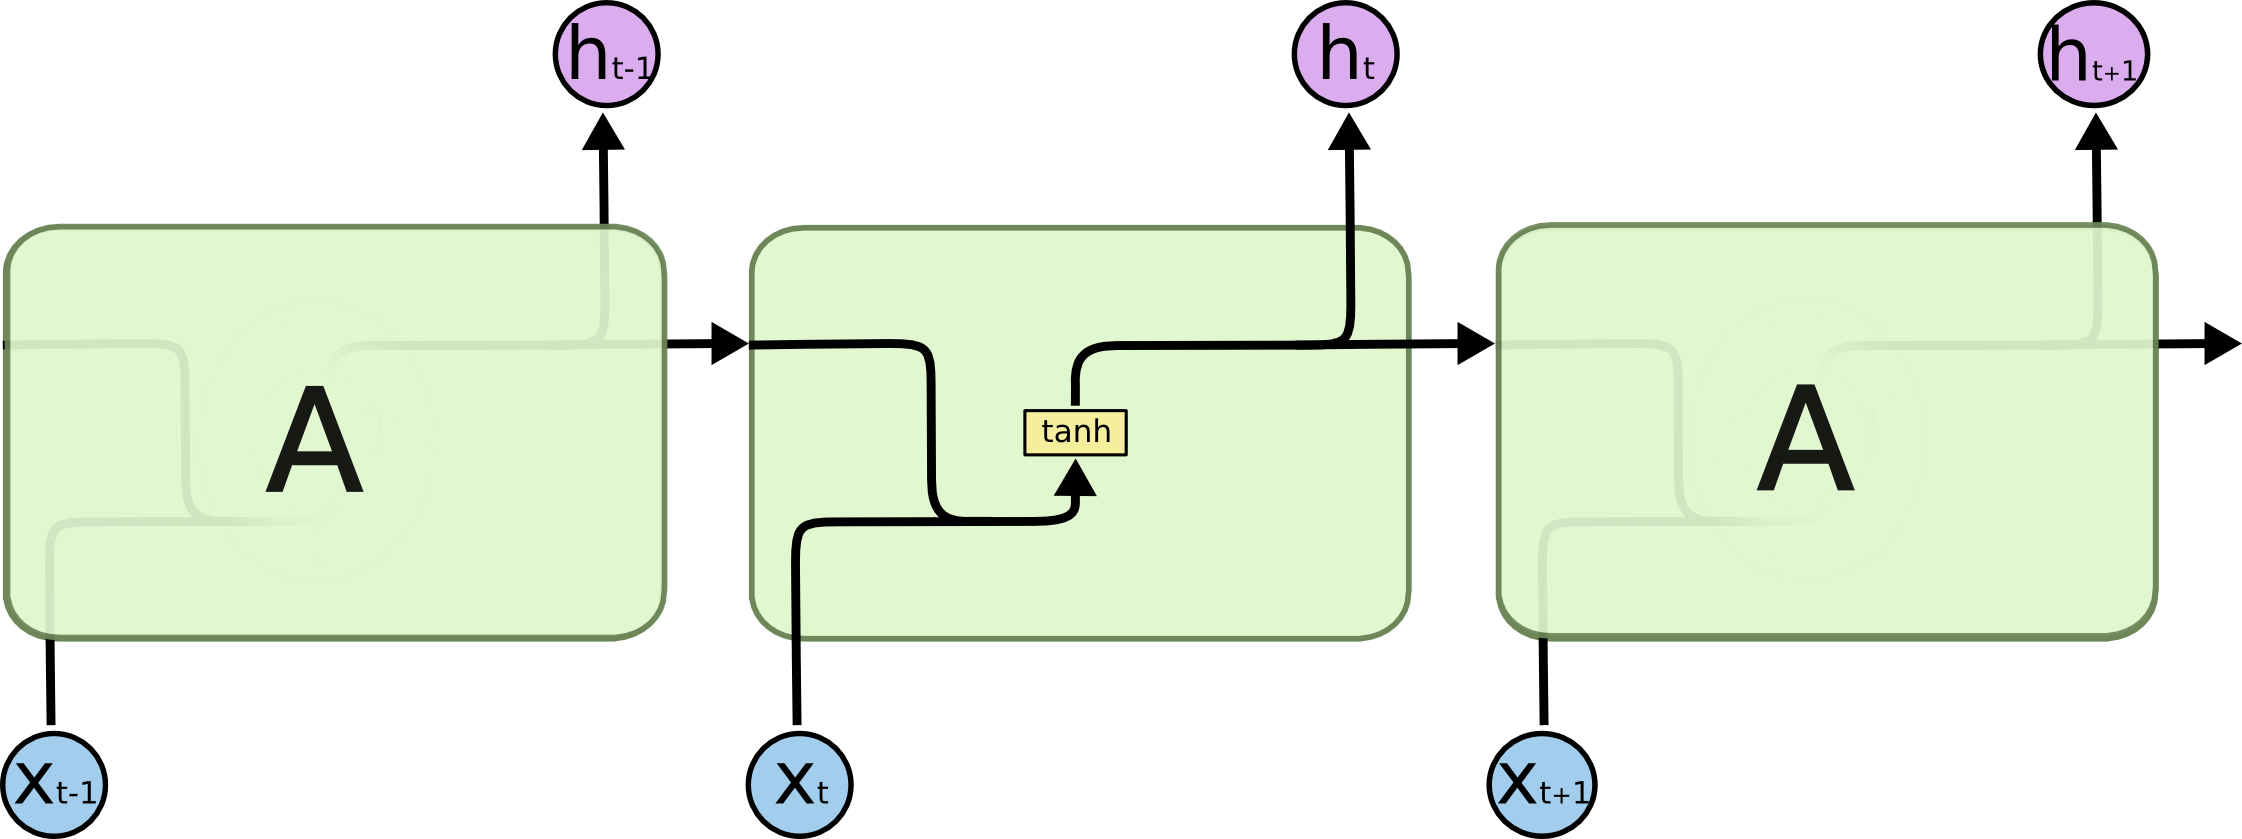
\includegraphics[width=0.9\textwidth]{Figures/LSTM3-SimpleRNN.png}
\decoRule
\caption[Red \glsentrytext{rnn} clásica]{Red \glsentrytext{rnn} clásica. Tomado de \cite{understanding-lstm}.}
\label{fig:rnn-classic}
\end{figure}

\begin{figure}[H]
  \centering
  % \missingfigure{Hacer la arquitectura en yEd}
  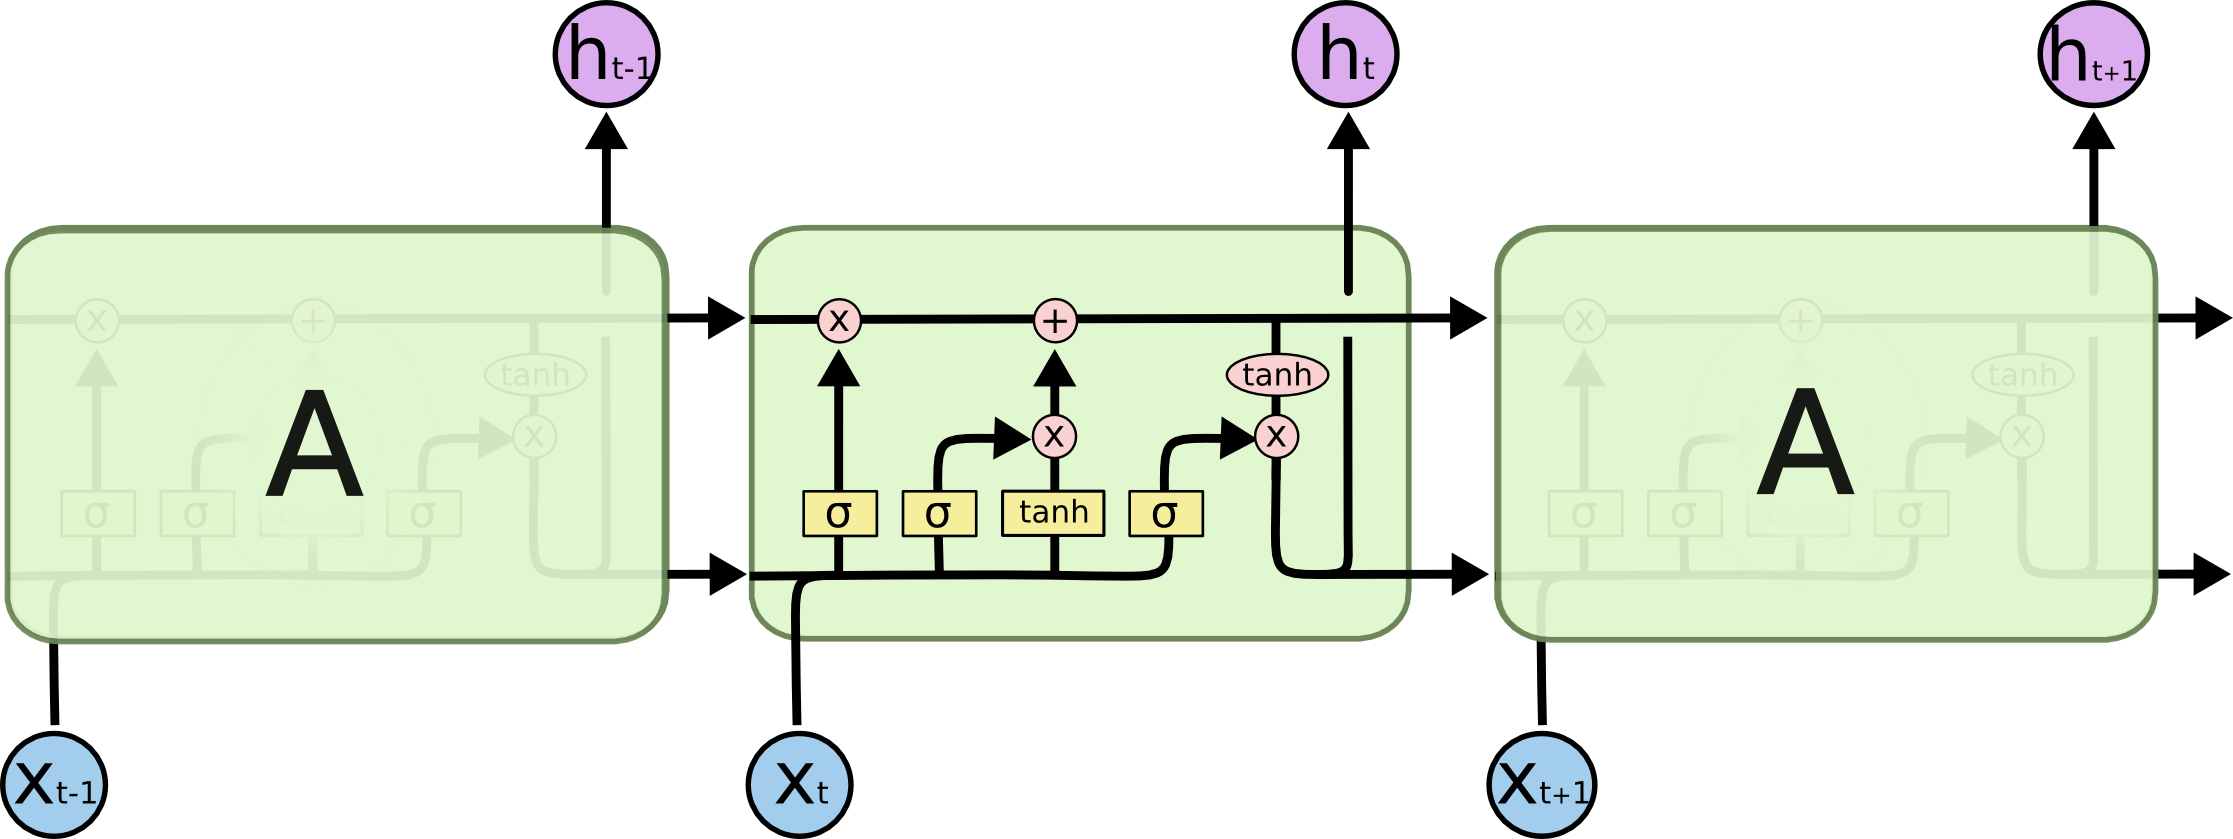
\includegraphics[width=0.9\textwidth]{Figures/LSTM3-chain.png}
\decoRule
\caption[Red \glsentrytext{lstm} clásica]{Red \glsentrytext{lstm} clásica. Tomado de \cite{understanding-lstm}.}
\label{fig:lstm-classic}
\end{figure}

\subsubsection{Redes neuronales \glsentrylong{bilstm}}
En la tarea de etiquetado de secuencias de texto las \gls{bilstm} tienen acceso a muestras de entrada tanto de pasado, presente y futuro por una cierta cantidad de tiempo. El uso de esta característica se puede aprovechar para ir a estados en el futuro (por medio de estados hacia adelante) y en el pasado (por medio de estados hacia atrás) para un momento particular en el tiempo \cite{Huang2015}.

Con el fin de que la red sea bidireccional es necesario de una celda de memoria para el caso de desplazarse hacia adelante, y una para desplazarse hacia atrás.

\subsubsection{Reconocimiento de \glsentrylong{namedent}}
Para el reconocimiento de \gls{namedent} tómese como ejemplo el \cref{table:namedent-example}, donde las etiquetas asignadas corresponden al reconocimiento correspondiente de cada entidad.
Las etiquetas (tags) de respuesta son \emph{Otro} (\textsc{O}) o una de estas: \emph{Persona} (\textsc{PER}), \emph{Ubicación} (\textsc{LOC}), \emph{Organización} (\textsc{ORG}) y \emph{Misceláneo} (\textsc{MISC}), donde las partes de etiqueta \textsc{B-} y \textsc{I-} corresponden a una palabra que se encuentra en la primera posición (\textsl{Beginning}) o en una posición intermedia (\textsl{Intermediate}).

\begin{table}[H]
  \centering
  \begin{tabular}{l|lllllll}
    \textbf{Texto}    & Donald   & Trump & es & presidente & de & Estados & Unidos \\
    \textbf{Etiqueta} & B-PER    & I-PER & O  & O          & O  & B-ORG   & I-ORG
  \end{tabular}
  \\ [1em]
  \decoRule
  \caption{Ejemplo de reconocimiento de \glsentrylong{namedent}.}
  \label{table:namedent-example}
\end{table}

La tarea de etiquetado para una \gls{lstm} y una \gls{bilstm} esta representada en la \cref{fig:lstm-arch} y la \cref{fig:bilstm-arch}.

\begin{figure}[H]
  \centering
  % \missingfigure{Hacer la arquitectura en yEd}
  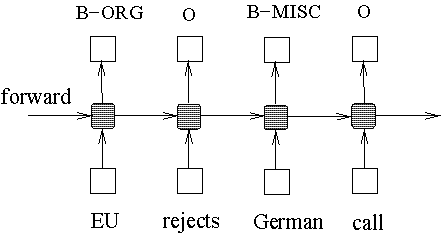
\includegraphics[width=0.6\textwidth]{Figures/lstm-arch.pdf}
\decoRule
\caption[Etiquetado con una \glsentrytext{lstm}]{Etiquetado con una \glsentrytext{lstm}. Tomado de \cite{Huang2015}.}
\label{fig:lstm-arch}
\end{figure}

\begin{figure}[H]
  \centering
  % \missingfigure{Hacer la arquitectura en yEd}
  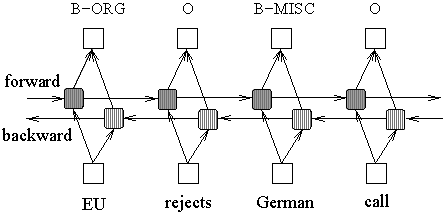
\includegraphics[width=0.6\textwidth]{Figures/bilstm-arch.pdf}
\decoRule
\caption[Etiquetado con una \glsentrytext{bilstm}]{Etiquetado con una \glsentrytext{bilstm}. Tomado de \cite{Huang2015}.}
\label{fig:bilstm-arch}
\end{figure}

\todo[inline]{Por favor explicar que ventaja tiene hacerlo con una BI-LSTM en lugar de una LSTM normal. En el caso de las figuras 6.8 y 6.9 los outputs son los mismos. ¿Este modelo (contribucion del pgr) se desarrollo finalmente como LSTM o BI-LSTM?}

% ================================================================

\subsubsection{Entrenamiento de \glsentrylong{bilstm}}
El entrenamiento de las redes \gls{bilstm} se empieza de manera similar a la descrita en la \cref{sec:twitter-prediction} con el procedimiento de asignar un identificador a cada \emph{token}\todo{Que es un token en este contexto? en la Seccion 6.3.1 no se mencionan tokens en ninguna parte} y a cada \emph{tag} como en las \cref{eq:lstm-token2id,eq:lstm-tag2id}, donde $N$ es el numero de tokens y $T$ el numero de tags. De manera que el conjunto de entrenamiento $\sX$ consta de tuplas $(\text{token}, \text{tag})$\todo{¿sería entonces un conjunto de tuplas (token, tag), que pueden ser: (<PAD>, tag1), (<UNK>, tag2)? No me queda claro que los tokens hagan parte del conjunto de datos de entrenamiento}, de donde se agregan dos tipos especiales de tokens\todo{Solo habrian estos 2 tipos de tokens?} \texttt{<PAD>} y \texttt{<UNK>}, que representan relleno y algo desconocido respectivamente.

\begin{equation} \label{eq:lstm-token2id}
  \text{token2id} = \Big\{(\text{token}_i, i) : \forall i \in \{1, \ldots, N\} \Big\}
\end{equation}

\begin{equation} \label{eq:lstm-tag2id}
  \text{tag2id} = \Big\{(\text{tag}_i, i) : \forall i \in \{1, \ldots, T\} \Big\}
\end{equation}

\paragraph{Generación de \textsc{Batches} para las redes \textsc{Bi-LSTM}}
Las redes neuronales son comúnmente entrenadas por grupos (o \emph{batches} en ingles) de entrada. Eso significa que las actualizaciones de los pesos dentro de la red se basan en secuencias en cada instante de tiempo. Pero estas secuencias dentro de un batch deben tener la misma longitud, así que estas se rellenaran con una etiqueta de relleno \texttt{<PAD>}. También es buena idea proveer la red con la longitud de las secuencias, para que así pueda saltarse computaciones innecesarias de las partes de relleno. A las partes de relleno se le asigna un tag de \texttt{O}.

\paragraph{Construcción de capas de la red neuronal}
Para esta construcción se procede a generar una matriz de \emph{embeddings} aleatorios, que en el caso de \gls{tensorflow} son tensores aleatorios y se establecen las células de procesamiento \emph{forward} y \emph{backward} con valores de marginalización\todo{por favor colocar que utilidad tienen estos valores de marginalizacion} $\xi$ (valor establecido heurísticamente) que es una forma de regularización importante en redes neuronales, de donde se especifica la probabilidad de retención\todo{es decir que la memoria depende de la probabilidad de retencion?} de los valores de la iteración anterior.

La salida de las celdas de \emph{forward} y \emph{backward} serán dos tensores $\tF$ y $\tB$, que se concatenan en un tensor $\tO$.\todo{esto se puede representar de manera visual?}

\paragraph{Computación de predicciones}
Se computa la función $\softmax$\todo{por favor explicar que hace la funcion softmax} sobre $\tO$ para convertir las entradas en una forma de probabilidad, de forma que se estan calculando las probabilidades de cada una de las entradas para luego calcular cuales son las entrada de mayor probabilidad, estimando así la predicción $P$, como se muestra en la \cref{eq:bilstm-pred}.

\begin{equation} \label{eq:bilstm-pred}
  P = \argmax_i (\softmax(\sigmoid(\tO_i)))
\end{equation}

Sin embargo, durante el entrenamiento no necesitamos una predicción, sino una función de perdida (o \emph{loss} en ingles), que se calcula como se muestra en la \cref{eq:cross-entropy-loss}, y en la \cref{fig:cross-entropy-y1}, donde $\hat{y}$ es la predicción y $y$ es el valor verdadero.

\begin{equation} \label{eq:cross-entropy-loss}
  \gamma(\hat{y}, y) = -{(y\log(\hat{y}) + (1 - y)\log(1 - \hat{y}))}
\end{equation}

\begin{figure}[H]
  \centering
  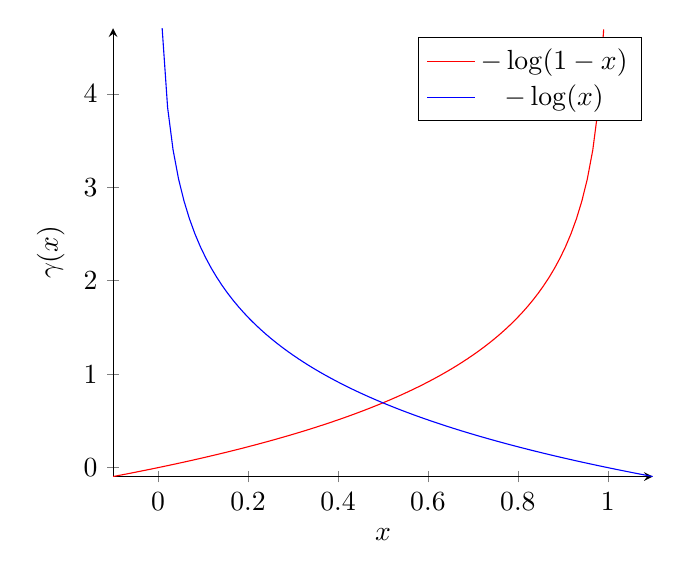
\begin{tikzpicture}
    \begin{axis}[
      axis lines = left,
      xlabel = $x$,
      ylabel = {$\gamma(x)$},
      ]
      % Below the red parabola is defined
      \addplot [
      domain=-0.1:1.1, 
      samples=100, 
      color=red,
      ]
      {-ln(1-x)};
      \addlegendentry{$-\log(1-x)$}
      % Here the blue parabloa is defined
      \addplot [
      domain=-0.1:1.1, 
      samples=100, 
      color=blue,
      ]
      {-ln(x)};
      \addlegendentry{$-\log(x)$}
    \end{axis}
  \end{tikzpicture}
\decoRule
\caption[Gráficas de cross-entropy]{Gráficas de cross-entropy (azul) si $y = 1$ (rojo) si $y = 0$.}
\label{fig:cross-entropy-y1}
\end{figure}

De manera que si se calcula una predicción de $\num{1e-8}$ cuando el valor verdadero es $1$, dará como resultado un valor alto de perdida (e.g. $\gamma(\num{1e-8}, 1) \approx \num{18.42}$).

Se calcula un tensor de perdida $\tL$ con $\softmax(\gamma(\sigmoid(\tO)))$, para luego calcular la media $\mu_{\tL}$ del tensor $\tL$. Y se pasa por una tensor mascara\todo{por favr explicar cual es la utilidad de este tensor mascara?} $\tM$ (\cref{eq:bilstm-mask-tensor}) que multiplica por $\tL$, donde $\train$ es el batch de entrenamiento. Entiéndase al tensor $\tM$ como el tensor que representa las posiciones que no son \texttt{<PAD>} con valor de $1$ y valor $0$ si lo son dentro del batch.

\begin{equation} \label{eq:bilstm-mask-tensor}
  \tM = \sum_{i \in \{1, \ldots, |\train|\}} \ve_{\mathrm{tag_i = \mathrm{PAD}}}^{(i)}
\end{equation}

Para realizar el entrenamiento con esta función de perdida se realiza una optimización (el optimizador estocástico \textsc{Adam} \cite{Kingma2014} es una opción eficiente\todo{explicar brevemente porque es eficiente?}) con una tasa de aprendizaje $\alpha$.

% ================================================================
% ================================================================
% ================================================================

\subsection{Modelo 3: Búsqueda de tweets relacionados con \emph{embeddings} de \mbox{StarSpace}}
En este modelo, la intención es que a partir de una colección de textos guardados en una base de datos se puedan obtener los $k$ textos mas similares a un texto de consulta $q$, de manera que se encuentren los textos de mayor similaridad en cuanto a las palabras usadas por medio del uso de \emph{embeddings}.

\todo[inline]{Por favor colocar aqui debajo un parrafo breve que represente la pregunta de data science que resuelve este modelo}

\subsubsection{?`Que son y como se usan los embeddings?}
Los \emph{embeddings} se pueden entender como vectores $n$--dimensionales que representan palabras dentro de un diccionario. Los modelos previamente vistos \gls{bow} y \gls{tfidf} se pueden entender como \emph{embeddings}, sin embargo para la aplicación en este modelo, es necesario otro \emph{embedding} que permita encontrar la similaridad entre palabras de forma que palabras que tengan un significado parecido tengan una distancia menor que si se comparara con una palabra que fuera antónima, de forma que $\mathrm{dist}(\vp_{\mathrm{asombroso}}, \vp_{\mathrm{genial}}) \gg \mathrm{dist}(\vp_{\mathrm{asombroso}}, \vp_{\mathrm{terrible}})$, donde $\mathrm{dist}$ típicamente seria la distancia de similaridad coseno (\cref{eq:cosine-similarity}).

\begin{equation} \label{eq:cosine-similarity}
  \mathrm{similaridad}(a, b) = \cos(\theta) = \frac{\vp_a \times \vp_b}{\norm{\vp_a} \norm{\vp_b}} \,,\, a, b \in d
\end{equation}

Dentro de los ejemplos de uso popular de \textit{embeddings} están \emph{GloVe} \cite{pennington2014glove}, \emph{word2vec} \cite{Mikolov2014}, \emph{fastText} \cite{joulin2016fasttext}, entre muchos otros.

\subsubsection{Calculo de vectores de varias palabras}
Una adición a las ventajas dadas por estos \emph{embeddings} es la capacidad de representar textos completos por medio de obtener la representación de cada termino (palabra) $t \in d$ y posteriormente calcular el promedio $\vs$ (\cref{eq:embeddings-sum}).

\begin{equation} \label{eq:embeddings-sum}
  \vs = \frac{1}{|d|} \sum_{t \in d} \vp_{t}
\end{equation}

\subsubsection{Evaluación de similaridad entre textos}
Nos podemos imaginar que usando un buen \emph{embedding} la similaridad coseno entre frases duplicadas\footnote{Entiéndase a una frase duplicada como textos que sean equivalentes ``semánticamente'' pero no necesariamente iguales sintácticamente} va a ser menor que para las frases aleatorias que generemos. Sobretodo que para cada par de frases duplicadas podemos generar $R$ ejemplos de frases negativas y encontrar la posición del texto duplicado correcto.

Sin embargo, no es buena idea considerar que el primer candidato sera siempre el primer resultado que dio la mayor similaridad, por lo que se tomara como una lista ordenada y se formulará una métrica de comparación. Podemos tomar a $K$ como un numero razonable de mejores elementos y $N$ el numero de consultas (tamaño de la muestra).

\paragraph{Métrica Hits@K}
La primera métrica que se usaría seria el numero de ``hits''\todo{que significa un hit correcto?} correctos para algún $K$, vea la \cref{eq:hits-k}.

\begin{equation} \label{eq:hits-k}
  \mathrm{Hits@K} = \frac{1}{N} \sum_{i=1}^{N} [\mathrm{dup}_i \in \mathrm{topK}(q_i)]
\end{equation}
Donde $q_i$ es la $i$--\'esima consulta, $\mathrm{dup_i}$ es su duplicado y $\mathrm{topK}(q_i)$ son los $K$ elementos mas similares provistos por nuestro modelo donde $[\mathrm{dup}_i \in \mathrm{topK}(q_i)]$ obtiene valor de $1$ si la condición que el duplicado este dentro de los $K$ elementos es verdadera y $0$ de lo contrario\footnote{A esta notación se le conoce como el paréntesis de Iverson (o \textsl{Iverson bracket} en inglés) \href{https://en.wikipedia.org/wiki/Iverson\_bracket}{wikipedia.org/wiki/Iverson\_bracket}}.

\paragraph{Métrica DCG@K}
La segunda métrica es conocida como \emph{Discounted cumulative gain} (versión simplificada), dada por la \cref{eq:dcg-k}.

\begin{equation} \label{eq:dcg-k}
  \mathrm{DCG@K} = \frac{1}{N} \sum_{i=1}^{N} \frac{1}{\log_2(1+\mathrm{rank}_{\mathrm{dup}_i})} [\mathrm{rank}_{\mathrm{dup}_i} \le K]
\end{equation}

Donde $\mathrm{rank}_{\mathrm{dup}_i}$ es la posición del duplicado en la lista ordenada de frases mas cercanas al texto de la consulta $q_i$. De acuerdo a esta métrica, el modelo obtiene una mayor recompensa por una posición mas alta de la respuesta correcta. Si la respuesta no aparece en $\mathrm{topK}$ en absoluto, entonces la recompensa es $0$.

\subsubsection{\glsentrylong{starspace}}
\gls{starspace} \cite{starspace} es un modelo neuronal de propósito general para el aprendizaje eficiente de \emph{embedding} de entidades para resolver una gran variedad de problemas, entre estas están:
\begin{itemize}
\item Aprendizaje de \emph{embeddings} a nivel de palabras, frases y documentos.
\item Obtención de información: ``ranking'' de conjuntos de entidades/documentos u objetos.
\item Clasificación de textos.
\item Aprendizaje de similaridad de textos.
\item Entre otras.
\end{itemize}

\paragraph{?`Como funciona y cual es la principal diferencia con \emph{word2vec}?}
\gls{starspace} puede ser entrenado específicamente para algunas tareas. En contraste con \emph{word2vec}, el cual intenta entrenar \emph{embeddings} similares para palabras en contextos similares, \gls{starspace} usa \emph{embeddings} para las frases completas (tal como la suma de los \emph{embeddings} para palabras y frases). A pesar de que se obtienen \emph{embeddings} en ambos casos como resultado del entrenamiento, los \emph{embeddings} de \gls{starspace} son entrenados usando datos supervisados.\todo{que ventaja hay en que el entrenamiento sea con datos supervisados?}

\subsubsection{Uso de \emph{embeddings} creados con \glsentrylong{starspace}}
En este caso, \gls{starspace} debería usar dos tipos de pares de secuencias para el entrenamiento: ``positivas'' y ``negativas''. Las muestras ``positivas'' son extraídas del conjunto de entrenamiento $\train$ (duplicados, alta similaridad) y las muestras ``negativas'' que son generadas aleatoriamente (se asume que tienen una baja similaridad).

De forma que se pueda usar \gls{starspace} es necesario primero compilar el código fuente provisto del repositorio de código de GitHub\footnote{\href{https://github.com/facebookresearch/StarSpace}{https://github.com/facebookresearch/StarSpace}} (Solo funciona MacOS o Linux). Se puede clonar el codigo fuente por medio de introducir los  comandos en la Terminal de la \cref{fig:starspace-terminal-compilation}.

\begin{figure}[ht]
\centering
\begin{minipage}{0.9\textwidth}
\begin{minted}[linenos,breaklines,fontsize=\footnotesize]{bash}
git clone https://github.com/facebookresearch/Starspace.git
cd Starspace
make
\end{minted}
\end{minipage}
\caption{Ejemplo en compilación de \glsentrylong{starspace} en la Terminal.} 
\label{fig:starspace-terminal-compilation}
\end{figure}

Para luego ejecutarlo con diferentes parámetros de entrada y un conjunto de entrenamiento en un archivo \texttt{.tsv}, como se muestra en la \cref{fig:starspace-terminal-execution}.

\begin{figure}[ht]
\centering
\begin{minipage}{0.9\textwidth}
\begin{minted}[linenos,breaklines,fontsize=\footnotesize]{bash}
starspace train -trainFile prepared_train.tsv -model modelSaveFile -trainMode 3 -adagrad 1 -ngrams 1 -epoch 5 -dim 100 -similarity cosine -minCount 2 -verbose 1 -fileFormat labelDoc -negSearchLimit 10 -lr 0.05
\end{minted}
\end{minipage}
\caption{Ejemplo en ejecución de \glsentrylong{starspace} en la Terminal.} 
\label{fig:starspace-terminal-execution}
\end{figure}

Donde se ejecuta a \gls{starspace} en modo de entrenamiento, tiene el archivo de entrenamiento (\texttt{prepared\_train.tsv})\todo{son datos etiquetados?}, el modo de entrenamiento para exploración de similaridad de textos (\texttt{-trainMode 3}), uso de optimización \textsc{Adagrad} (\texttt{-adagrad 1}), con n-gramas de tamaño $1$ (\texttt{-nrams 1}), $5$ iteraciones (\texttt{-epoch 5}), vectores resultantes en $\R^{100}$ (\texttt{-dim 100}), uso de similaridad coseno (\texttt{-similarity cosine}), conteo mínimo de $2$ términos (útil si no se quieren obtener \emph{embeddings} de palabras extremadamente raras, \texttt{-minCount 2}), numero mínimo de ejemplos negativos como $10$ usado durante el entrenamiento (\texttt{-negSearchLimit 10}) y una tasa de aprendizaje de $0.05$ (\texttt{-lr 0.05}).

Luego de esto el resultado es un archivo de \emph{embeddings}, donde cada linea esta compuesta de una palabra y los $100$ números que componen al vector de esa palabra.

Estos \emph{embeddings} resultantes permiten luego realizar la obtención de los $k$ textos mas similares a un tweet de consulta $q_i$ obtenido de \emph{pool} de textos obtenidos de Twitter de fuentes relevantes de forma que se encuentren textos relacionados a individuos que tuvieran relación con grupos terroristas.

% ================================================================
% ================================================================
% ================================================================

\section{Despliegue (Deployment)}
A la fecha, los productos disponibles para el despliegue son el primer modelo propuesto (\cref{sec:twitter-prediction}), una implementación del meta-modelo \gls{som} (\cref{subsec:SOM}) y la implementación de la recolección de información de tweets (\cref{sec:data-acquisition}).

